\documentclass[12pt,titlepage]{article}
\usepackage{comment}
\usepackage[margin=1in]{geometry} 
\usepackage{amsmath}
\usepackage{tcolorbox}
\usepackage{amssymb}
\usepackage{amsthm}
\usepackage{lastpage}
\usepackage{fancyhdr}
\usepackage{accents}
\usepackage{enumerate}
\usepackage{graphicx}
\usepackage{siunitx}
\usepackage{mhchem}
\usepackage{tikz}
\usepackage{xcolor}
\usepackage{titling}
\usepackage{draftwatermark}
\usepackage{hyperref}
\usepackage[shortlabels]{enumitem}
\pagestyle{fancy}
\setlength{\headheight}{40pt}

\newenvironment{solution}
  {\renewcommand\qedsymbol{$\blacksquare$}
  \begin{proof}[Solution]}
  {\end{proof}}
\renewcommand\qedsymbol{$\blacksquare$}

\newcommand{\ubar}[1]{\underaccent{\bar}{#1}}

\newtheorem{lemma}{Lemma}

\definecolor{meablue}{HTML}{0160E2}
\definecolor{meared}{HTML}{BE3751}

\graphicspath{ {./assets/} }
\SetWatermarkAngle{0}
\SetWatermarkText{
\includegraphics[scale=0.3]{watermark.png}}

\hypersetup{
  colorlinks=true,
  urlcolor=blue
}

\predate{}
\postdate{}

\preauthor{}
\postauthor{} % add packages, settings, and declarations in settings.tex

\begin{document}

\sffamily

\DraftwatermarkOptions{stamp=false}

\lhead{\textsf{\textbf{\textcolor{meablue}{Math et al}}}} 
\rhead{\textsf{\textcolor{meared}{1st} Anniversary Contest}} 
\cfoot{\thepage\ of \pageref*{LastPage}}
\title{
\includegraphics[scale=0.3]{favicon.png} \\ \textbf{\textcolor{meablue}{Math et al's}} \\ 1st Anniversary Contest}
\date{}
\author{}
\titlepage
\maketitle

\DraftwatermarkOptions{stamp=true}

\section*{\textsf{\textbf{Format}}}
There will be 5 Math and 5 Physics problems, some with subquestions. The difficulty of both sections range from low AIME/F=ma to low Olympiad level. Participate in teams up to 2.
\\ \\
Problems are proof by default, you must provide a full solution; a final answer by itself is worth nothing. However, you may provide solely the final answer to problems marked by an asterisk (*). Part marks may be given for incomplete progess, including on * problems, so submit what you have.
\\ \\
The maximum possible amount of points awarded for each problem is given in the document. Your team's final score is the sum of the points attained over all problems. Problems are generally sorted in increasing order of difficulty.
\\ \\
Both pictures of handwritten solutions and \textrm{\LaTeX} pdfs are accepted. Handwritten solutions should be clear and legible.
\\ \\
All questions are original and made by our staff. Enjoy!
\\ \\
\textbf{Submit here: \url{https://forms.gle/3eKUtoU5zhuv12k78}}

\section*{\textsf{\textbf{Rules}}}
\begin{itemize}
    \item Calculator allowed for basic arithmetic calculations only
    \item No resources allowed (internet, books, WolframAlpha etc)
    \item No communication about the problems with anyone other than teammate(s)
    \item Both members must be in the \href{https://mathetal.org/discord}{Math et al Discord Server}!
\end{itemize}

\section*{\textsf{\textbf{Acknowledgements}}}
Math et al would like to thank the RedSuns and FISKON communities for their support! Additionally, thanks to Jeli, BariumLanthanum, TheCelestialCube, and Polarity/TropicoMango for making the problems.

\newpage 

\begin{comment}
    {[4 points]} Mango recieved some presents for the anniversary, including an $m$ times $n$ grid, for positive integers $m, n$ that satisfy $4 \mid mn$. The grid comes with a supply of tetrominoes.
        \begin{figure}[!ht]
            \centering
            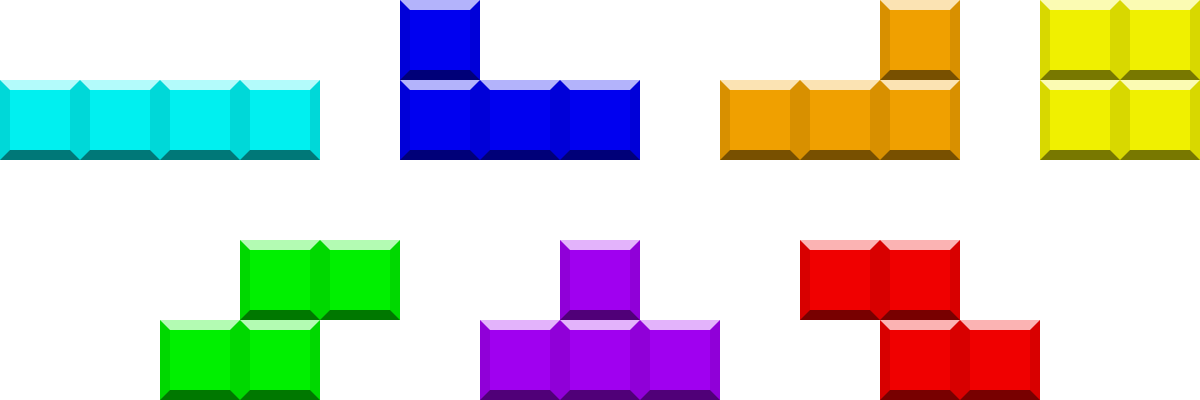
\includegraphics[scale=0.2]{tetrominoes.png}
            \caption{The seven types of tetrominoes}
        \end{figure}
        \\ Mango tiles the grid using some tetrominoes (possibly rotated) such that:
        \begin {itemize}
        \item Each of the four individual cells in each tetromino overlap perfectly with some cell in the grid
        \item Each cell in the grid is covered by some tetromino
        \item No two tetrominoes overlap
        \end {itemize}
        Prove that the \emph{T} (purple) tetromino is used an even amount of times in the tiling.
\end{comment}


\section*{\textsf{\textbf{\textcolor{meablue}{Math}}}}
\begin{enumerate}[align=left,start=1,label=\textbf{\textcolor{meablue}{Problem \arabic*}}]
    \item {[$4$ points*]} Concentric circles $\omega_1$ and $\omega_2$ are centered at $O_1$ and have radii of $5$ and $13$, respectively. A third circle $\omega_3$ centered at $O_2$ is externally tangent to $\omega_1$ and intersects $\omega_2$ at $M$ and $N$. Let $P$ be the point on $\omega_2$ such that $PO_1$ is perpendicular to $O_1 O_2$ and is closer to $M$ than $N$. If $PN$ is tangent to $\omega_1$, then the radius of $\omega_3$ is $\frac{m}{n}$ for relatively prime positive integers $m, n$. Find $m + n$.
    \item {[$5$ points]}
        As a present for the anniversary, Mango recieved an $m$ times $n$ (for positive integers $m, n$) chess board, along with some tokens. He places some tokens in the board (each cell can contain \emph{any amount} of tokens). Mango observes that the total amount of tokens in each row and each column is even. Prove that there are an even number of tokens that are in white cells.
    \item {[$6$ points]} Find all solutions in rational numbers $(x, y, z)$ such that
        \[x + \sqrt[3]{3}y + \sqrt[3]{9}z = 0\]
    \item 
        Cubbo is playing a board game called \emph{Threetris}, which he recieved as a present for the anniversary. The game is played on a well designed rectangular board, with each of its \emph{four edges colored a different color}. Engraved into the board is a 3 times $N$ grid (for positive integer $N > 3$).
        \begin{figure}[!ht]
            \centering
            \begin{tikzpicture}[level/.style={sibling distance=50mm/#1},baseline=(current bounding box.north)]
                \draw[very thick] (1,1) -- (1,3);
                \draw[very thick] (1,1) -- (3,1);
                \draw[very thick] (1,3) -- (2,3);
                \draw[very thick] (3,1) -- (3,2);
                \draw[very thick] (2,3) -- (2,1);
                \draw[very thick] (3,2) -- (1,2);
                
                \draw[very thick] (4,2) -- (7,2);
                \draw[very thick] (4,1) -- (7,1);
                \draw[very thick] (4,1) -- (4,2);
                \draw[very thick] (5,1) -- (5,2);
                \draw[very thick] (6,1) -- (6,2);
                \draw[very thick] (7,1) -- (7,2);
            \end{tikzpicture}
            \caption{The two types of trominoes (long tromino on the right)}
        \end{figure}
        
        Cubbo is trying to place trominoes (possibly rotated) onto the grid such that:
        \begin {itemize}
        \item Each of the three individual cells in each tromino overlap perfectly with some cell in the grid
        \item Each cell in the grid is covered by some tromino
        \item No two trominoes overlap
        \item All long trominoes must be placed parallel to the board edges of grid length 3, as Cubbo, being very short, is jealous of the long tromino's height.
        \end {itemize}
        
    \begin{enumerate}
        \item {[$2$ points*]} Let $T(N)$ denote the number of ways of distinct tilings to satisfy Cubbo's requirements, on a 3 times $N$ Threetris board. Help Cubbo find $T(10)$.
        \item {[$5$ points*]} Let $\mathcal{T}(n)$ denote the largest nonnegative integer $t$ such that $3^t \mid n$, for positive integer $n$. A \emph{Threetastic} number $x$ is an \emph{even} positive integer satisfying:
        \begin{itemize}
            \item $x$ has less than 3 prime divisors. 
            \item $x$ has less than $10^3$ positive integer divisors. 
            \item $\mathcal{T}(T(x))$ is divisible by 2022
        \end{itemize}
        
        Find the number of \emph{Threetastic} numbers.
    \end{enumerate}
    \item {[$8$ points]} On an infinitely long railroad from west to east, $n$ trains cars, some containing dynamite, start evenly spaced and all move due east at distinct constant speeds. When one train $A$ catches up to another train $B$, $A$ slows down and the front of $A$ connects to the back of $B$ to become a longer train. Train cars by themselves are also considered a train. Note the number of train cars in this longer train is the number of train cars in $A$ plus the number of train cars in $B$, and the longer train continues moving at the same speed as $B$. After a long time has passed (such that no new train connections will take place), the trains halt and are inspected. A train is \emph{safe} if it has two consecutive train cars both not containing dynamite, otherwise it is \emph{dangerous}. All dangerous trains are removed from the track due to safety hazards, and the total amount of removed \emph{train cars} is $N$. Derive an expression in $n$ for the expected value of $N$. 
\end{enumerate}
 
\newpage 
\DraftwatermarkOptions{stamp=false}

\section*{\textsf{\textbf{\textcolor{meared}{Physics}}}}
Numerical answers can be rounded to one decimal place. Physics constants can be found \href{https://en.wikipedia.org/wiki/List_of_physical_constants}{here}.
\begin{enumerate}[align=left,start=1,label=\textbf{\textcolor{meared}{Problem \arabic*}}]
    \item {[$4$ points*]}
        Anduwu is driving a car with an open rectangular container of milk inside. The container is $6$ inches long, $6$ inches wide, and $5$ inches high, containing milk $3$ inches high when level. He encounters a circular curve on the highway with a radius of $\qty{200}{\meter}$, and one side of the milk container remains parallel to the car's velocity throughout the curve. Assume the milk has negligible viscosity, the car has negligible body roll, and the coefficient of static friction between the tires and road is $1.6$. Whats the fastest speed Anduwu can travel at, while having the car neither slip nor spill the milk?
    \item {[$5$ points*]} 
         A certain scientific railgun with mass $\qty{10000}{\kilo\gram}$ stationed in deep space (negligible gravity from outside the system) uses an electric charge to shoot a coin-shaped projectile, which is accelerated by the electrical potential difference. The coin is shot directly toward a stationary target practically infinite distance away. The coin has a mass of $\qty{10}{\kilo\gram}$ and a positive charge of $\qty{1}{\micro\coulomb}$. Inside the railgun there is a sphere of positive charge $N\,\unit{\coulomb}$. If the coin hits the target at $\qty[per-mode = symbol]{2000}{\meter\per\second}$, what is the value of $N$?
    \item
        Bala is conducting an interesting experiment with a special cubic device shipped from Brazil. This device is a lightweight cube with a mass of $\qty{2}{\gram}$, with each face having a purely cosmetic label as shown in the diagram.
        \begin{figure}[!ht]
            \centering
            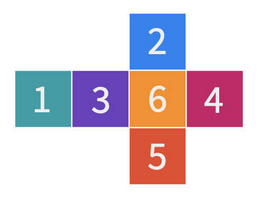
\includegraphics[scale=0.6]{cube.png}
            \caption{Net of the cubic device}
        \end{figure}
        The cube continuously emits red, blue, or green light on exactly three specific faces, with each such face emitting photons perpendicular to the face. He places the cube on a large flat frictionless surface with the face labelled \emph{2} facing directly north and face \emph{1} pointing upward. The cube moves without any external force and solely from emitting light at a power of \qty{20}{\watt} per light emitting face. Bala records its motion using his favorite Lenovo Thinkpad. When he starts the experiment, all of the light emitting faces emit red light. After $3$ hours, they all start emitting blue light, and then after $3$ hours again they all emit green light, and red light again and the loop repeats. After $7$ hours of the experiment, Bala measures that the cube has an instantaneous velocity of $v = \qty[per-mode = symbol]{0.848}{\meter\per\second}$, directly southeast. 
        \begin{enumerate}
            \item {[$2$ points]} Find all possible combinations of the $3$ light emitting faces.
            \item {[$4$ points]} What is the velocity of the cube after $5$ hours had elapsed since the start of the experiment?
        \end{enumerate}
    \item {[$7$ points]}  
        A cylindrical vessel of height $h$ and radius $r$ is two-thirds filled with liquid. It is rotated with constant angular velocity $\omega$ about its axis, which is vertical. Neglecting any surface tension effects, find an expression for the greatest angular velocity of rotation $\Omega$ for which the liquid docs not spill over the edge of the vessel.
    \item 
        In Jeli's experiment, a cubical glass made up of Silicon dioxide (\ce{SiO_2}) is launched with an initial velocity of $\qty[per-mode = symbol]{10}{\meter\per\second}$. Then, it collides with a spring with a spring constant of $\qty[per-mode = symbol]{25}{\newton\per\meter}$ and compresses the spring to a maximum compression of $\qty[per-mode = symbol]{0.05}{\meter}$. During the compression, the glass cannot withstand such a resisting force and cracks are produced on the glass. The dimensions of the glass are $\qtyproduct{4 x 10 x 2}{\centi\meter}$.

        Constants:
        \begin{itemize}
            \item Density of glass: $\rho_{\ce{SiO_2}} = \qty[per-mode = symbol]{2}{\gram\per\centi\meter\tothe{3}}$
            \item Molecular mass of \ce{SiO_2}: $M_{\ce{SiO_2}} = \qty[per-mode = symbol]{60}{\gram\per\mole}$
            \item Latent heat of vaporization for glass: $L_g = \qty[per-mode = symbol]{10}{\kilo\joule\per\gram}$
        \end{itemize}

        \begin{figure}[!ht]
            \centering
            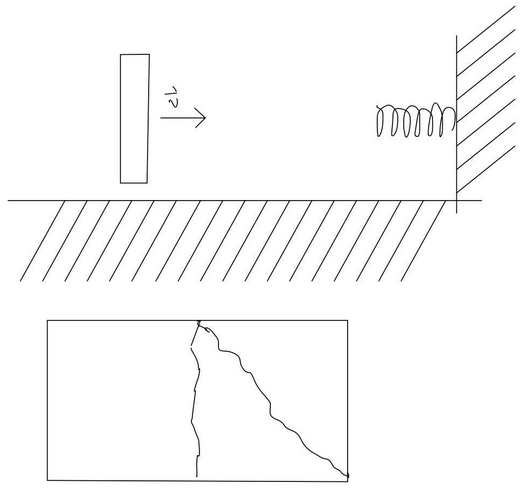
\includegraphics[scale=0.5]{physics5.png}
            \caption{Glass, spring, and the resulting two cracks}
        \end{figure}

        \begin{enumerate}
            \item {[$2$ points]} Using the figure, estimate the total length of cracks and the total number of broken bonds.
            \item {[$3$ points]} Using the latent heat of vaporization, estimate the bonding energy of glass.
            \item {[$3$ points]} Find the percentage of the energy lost in this collision (energy that doesn`t convert into either energy of breaking the bonds or spring potential energy).
        \end{enumerate}
\end{enumerate}

\end{document}